
\documentclass{article}
\usepackage{graphicx}
\usepackage{blindtext}
\usepackage{biblatex}
\usepackage{authblk}
\usepackage{titling}


\usepackage[a4paper, total={6in, 9.5in}]{geometry}

\begin{document}
	\section*{Define the problem} 
	Skin cancer is a dangerous and widespread disease [1] Each year there are approximately 5.4 million new cases of skin cancer are recorded in the USA alone [2], [4]. The global statistics are equally alarming [3][5]. Recent reports show that from 2008 to 2018, there has been a 53\% increase in new melanoma cases diagnosed annually [1,4]. The mortality rate of this disease is expected to rise in the next decade. The survival rate is less than 14\% if diagnosed in later stages.\\
	\section*{Dataset}
	The dataset was generated by the International Skin Imaging Collaboration (ISIC) and images are from the following sources: Hospital Clínic de Barcelona, Medical University of Vienna, Memorial Sloan Kettering Cancer Center, Melanoma Institute Australia, University of Queensland, and the University of Athens Medical School.
	\\
	\begin{center}
	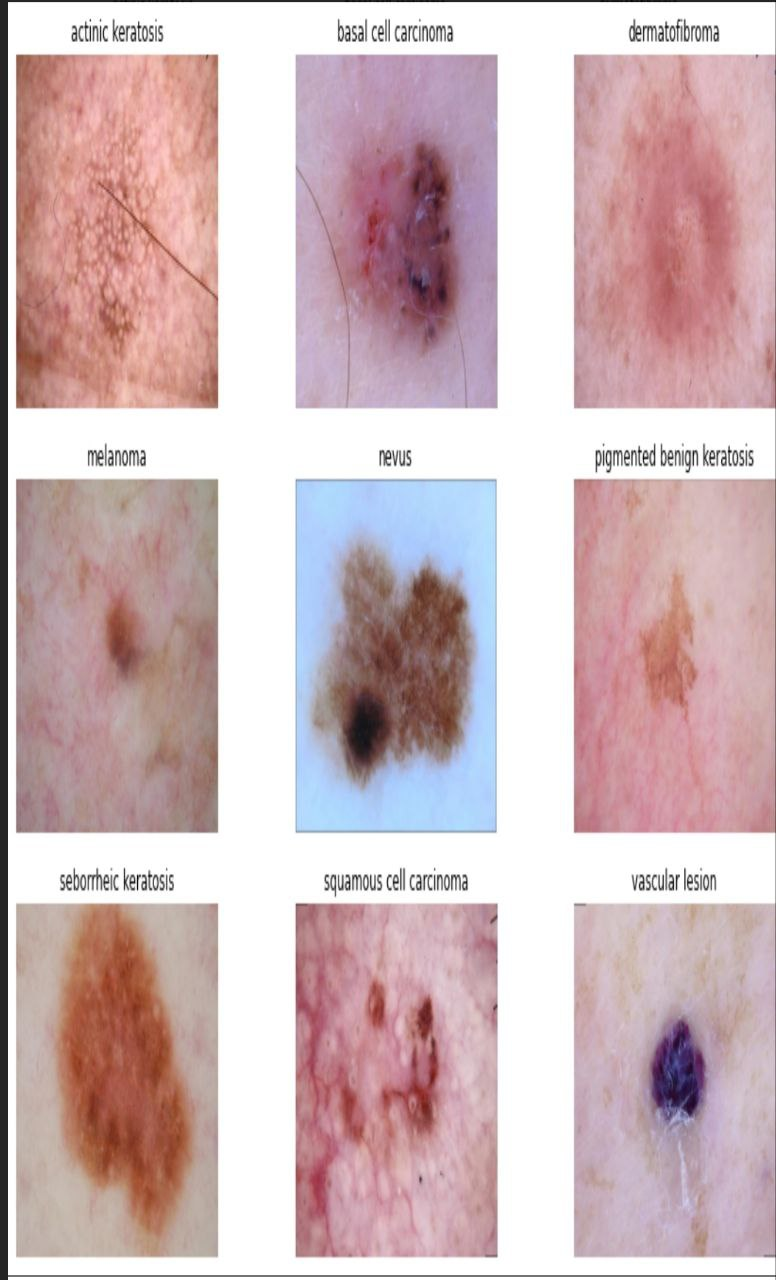
\includegraphics[scale=0.2]{./Fig/sample_photo.jpg}
	\end{center}
	\section*{Input \& Output}
	Developing a DeepLearningmodel to classify skin cancer images
	into 9 different categories with high enough accuracy to be
	reliable. Those categories are
	\begin{itemize}
		
	\item actinic keratosis 
	\item basalcellcarcinoma 
	\item dermatofibroma 
	\item melanoma 
	\item nevus 
	\item Pigmentedbenignkeratosis
	\item seborrheic keratosis 
	\item squamouscellcarcinoma 
	\item vascular lesion
	\end{itemize}
	
	\section*{Motivation}
	If skin cancer is detected at early stages then the survival rate is nearly 97\% [3]. This demands the early detection of skin cancer. This paper addresses the issue of early diagnosis, with improved accuracy.
	\\
	It is found that a skilled dermatologist usually follows a series of steps, starting with the naked-eye observation of suspected lesions, then dermoscopy (magnifying lesions microscopically), and followed by a biopsy. This would consume time and the patient may advance to later stages. Moreover, accurate diagnosis is subjective, depending on the skill of the clinician. It is found that the best dermatologist has an accuracy of less than 80\% incorrectly diagnosing skin cancer. Adding to these difficulties, there are not many skilled dermatologists available globally in public healthcare.
	\\
	
	To diagnose skin cancer speedily at the earliest stage and solve some of the aforementioned problems, there have been extensive research solutions by developing computer image analysis algorithms. The majority of these algorithmic solutions were parametric, meaning that they required data to be normally distributed. As the nature of data cannot be controlled, these methods would be insufficient to accurately diagnose the disease. However, non-parametric solutions do not rely on the constraint that the data is in normal distribution form.
	\\
	Our Model augmented assistance to the dermatologist is provided using deep learning. The essence of the approach is that a computer is trained 
	to determine the problem by analyzing the skin cancer images.\\
	
	\textbf{What makes it difficult?}
	\begin{itemize}
		\item Working with Multi-Class is not easy for getting good accuracy.
		\item Not Available Large Datasets.
		\item Datasets are available imbalanced.
		\item The distribution of data is not good.
	\end{itemize}
	\textbf{Related work:}\\
	What has been done? 
	The paper we used relied on VGG-16 which resulted in an accuracy of 69.57\% while the theVGG-19 had a better accuracy of 71.19\%
	The paper also did some preprocessing on the images such as
	Augmentationsetting Range \\
	\begin{center}
		\begin{tabular}{ccc}
			rotation range       &&        90 \\
			shear range            &&      0.1\\
			zoom range               &&   0.14 \\
			horizontal flip            &&    True\\
		\end{tabular}\\
	\end{center}
	\subsection *{What are the problems?}
		
	\begin{itemize}
		\item they both resulted in a model of a bigger size and used a padding 0
		\item which resulted in an image with fewer features in this particular
		model. 
		\item They are more attention to models than distribution data.
		
	\end{itemize}
	 \textbf{Working about data:}
		 
	 \begin{itemize}
	 	\item Datasets  4600 images, which is very small for 9 class, in addition, data is imbalanced and have very bad distribution.
	 	So, We working to solve this.
	 	\item Firstly, we split data into two partitions final set \& train set, then worked in data training to increase images and slove distribution.
	 	\item We making Augmentation using 
	 	Python package is known as Augmentor (https://augmentor.readthedocs.io/en/master/) to add more samples across all classes so that none of the classes have very few samples
	 	\item Instantiate a Pipeline object pointing to a directory containing your initial image data set.
	 	Define several operations to perform on this data set using your Pipeline object.
	 	Execute these operations by calling the Pipeline’s sample() method.
	 	\item Finally, we split data training to train \& validation, we worried that this approach makes overfitting, so, we split from data partition to data set	 	
	\end{itemize}
	\section* {Algorithm}
	\begin{itemize}
		\item We Used  Xception \&  inceptionv3  because the two algorithms use padding the same as it is suitable for our data and utils suitable resources, not as VGG.
		\item Our data is not very large, so transfer learning is a very good option, we do not make unfreeze layer also this problem dissimilar problem, but we used it as an initial weight instead of 
		We use Random initial weight, this option gives us a good result.
		\item Also, we added some layers
		\begin{itemize}
			\item GlobalAveragePooling2D
			\item Dropout
			\item BatchNormalization
			\item Dense
		\end{itemize}
		
		\item Using optimizers Adam with learning\_rate= 3e-4
		\item Using callbacks with 
		\begin{itemize}
			\item early stopping 
			\item ReduceLROnPlateau to reduce the learning rate the confusion metric has stopped improving. 

		\end{itemize}
		\item Xception accuracy with 
		\begin{itemize}
			\item Validation 94
			\item final test 91  
		\end{itemize}

		\item inceptionv3 accuracy with 
		\begin{itemize}
			\item Validation 91
			\item final test 88
		\end{itemize}
		So, we select Xception
	\end{itemize}
	\section*{Evaluation}
	\begin{itemize}
		\item We used the classification report to show the precision, recall, F1 Score, weighted average, and micro average.
		\item We used confusion\_matrix in the final test to know the conflict with classes
	\end{itemize}
	\pagebreak
	
	\begin{center}
		\textbf{Validation Result} \\
		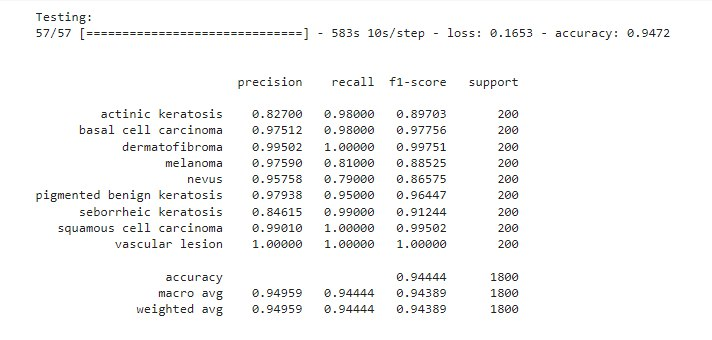
\includegraphics[scale=0.9]{./Fig/validation_reslut.jpg}
	\end{center}

	\begin{center}
		\textbf{Final Test} \\
		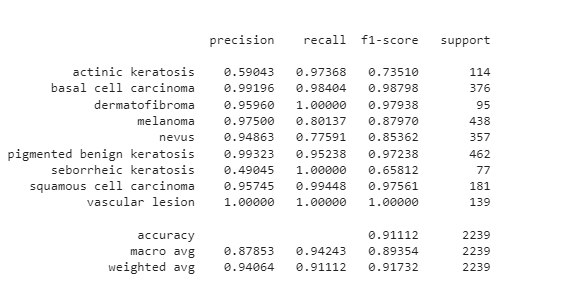
\includegraphics[scale=0.9]{./Fig/validation_test.jpg}
	\end{center}

	\begin{center}
		\textbf{Confusion Matrix in the final test} \\
		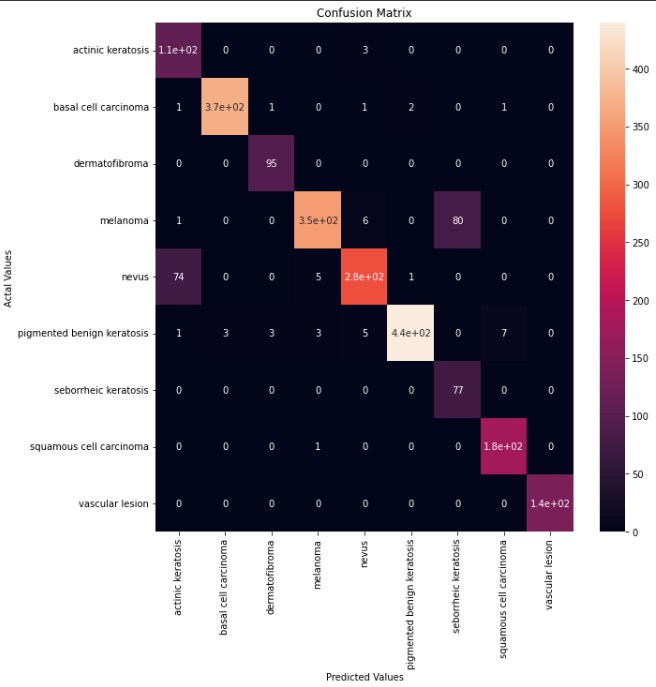
\includegraphics[scale=0.6]{./Fig/confiuson_matrix.jpg}
	\end{center}
	\section*{Analysis} 
	
	\begin{itemize}
		\item Our results are very good with another solution, but not very good for the medical field.	
	\end{itemize}
	We Noticed, Model, did not good t0 difference between:
	
	\begin{itemize}
		\item Actinic \& Nevus
		\item seborrheic keratosis \& melanoma
	\end{itemize}
	In our future, the plan is to work around data to solve this problem
	\begin{itemize}
		\item Our solution we working on using some preprocessing in data to solve this conflict.
		\item Another solution, make our system consist of two layers and merge Actinic \& Nevus in one category and seborrheic keratosis \& melanoma in one category, and layer two have two models of binary classification if the result is one of the merged categories, the disadvantage will resources usages
		
	\end{itemize}
	
	
	\section*{. Contribution}
		\begin{itemize}
			
			\item \textbf{Mohamed Badr}-sec 7
			\item \textbf{Abdullah Alqasabi}-sec 5 	
			\item \textbf{Abdelrahman Khaled}-sec 4 
			\item \textbf{Omar Adel Hassanen}-sec 5
			\item \textbf{Ibrahem Abd-Alatef}-sec 1
			
			
		\end{itemize}
	
	 

		
	
	
	

\end{document}
	
	
	
	
